\documentclass[12pt,letterpaper,final]{article}

\usepackage{Sweave}
\usepackage{graphicx}
\usepackage{natbib}
\usepackage{hyperref}
\usepackage{caption}
\usepackage{rotating}
\usepackage{verbatim}
\usepackage{textcomp}
%\usepackage[hyphens]{url}
\usepackage{latexsym}
\usepackage{wasysym}

\setlength{\oddsidemargin}{0in}
\setlength{\textwidth}{6.15in}
%\setlength{\topmargin}{0.5in}
\setlength{\textheight}{22cm}
\setlength{\headheight}{0in}
\setlength{\headsep}{0in}
\setlength{\parskip}{5pt plus 2pt minus 3pt}

\def\thefootnote{\fnsymbol{footnote}}
\setcounter{footnote}{1}

\renewcommand{\baselinestretch}{1.2}
\renewcommand{\labelenumi}{(\roman{enumi})}

\renewcommand{\topfraction}{1.0}
\renewcommand{\bottomfraction}{1.0}
\renewcommand{\textfraction}{0.0}
\renewcommand{\floatpagefraction}{1.0}

\newtheorem{definition}{Definition}
\newtheorem{theorem}{Theorem}
\newtheorem{lemma}[theorem]{Lemma}
\newtheorem{claim}[theorem]{Claim}
\newtheorem{fact}[theorem]{Fact}

% to get nice proofs ...
\newcommand{\qedsymb}{\mbox{ }~\hfill~{\rule{2mm}{2mm}}}
\newenvironment{proof}{\begin{trivlist}
\item[\hspace{\labelsep}{\bf\noindent Proof: }]
}{\qedsymb\end{trivlist}}


\newfont{\msymb}{cmsy10 scaled 1000}

\def\nullset{\mbox{\O}}
\def\R{{I\!\!R}}
\def\C{{I\!\!\!\!C}}
\def\N{{I\!\!N}}

\def\P{\mbox{\msymb P}}


%\parskip 0.1in
\pagenumbering{arabic}    %  Start using 1,2,... as page numbers.
\pagestyle{plain}         %  Page numbers in middle bottom of page.
%\setcounter{page}{80}  % XXXXXXXXXXXXXXXXX
%\setcounter{theorem}{5} % XXXXXXXXXXXXXXXXX
%\setcounter{definition}{10} % XXXXXXXXXXXXXXXXX

\parindent 0in


\begin{document}

\Sconcordance{concordance:hw03_bartschi.tex:hw03_bartschi.Rnw:%
1 161 1 1 2 1 0 5 1 1 5 11 0 1 9 8 0 1 1 4 0 1 2 8 1 1 8 7 0 1 3 2 0 1 %
1 12 0 1 1 4 0 1 2 7 1 1 3 14 0 1 2 1 0 2 1 1 4 3 0 1 3 1 0 1 1 1 3 1 0 %
1 3 1 0 1 4 3 0 1 2 12 0 1 2 9 1 1 3 2 0 1 11 13 0 1 2 14 1 1 2 1 0 1 %
48 51 0 1 2 34 1 1 3 2 0 1 1 1 3 2 0 3 1 5 0 1 1 1 2 1 0 2 1 1 2 1 0 1 %
4 2 0 2 1 1 8 6 0 2 2 1 0 1 1 1 2 1 0 1 5 1 0 1 8 6 0 2 1 1 2 1 4 2 0 3 %
1 1 3 1 0 1 4 1 0 2 3 1 0 1 3 1 0 1 9 12 0 1 4 2 0 1 8 6 0 1 3 1 8 10 0 %
1 2 213 1}


\begin{titlepage}
\vspace*{4.5cm}
\begin{center}
{\LARGE \bf Stat 5810, Section 003} \\[0.5cm]
{\LARGE \bf Statistical Visualization II} \\[0.5cm]
{\LARGE \bf Spring 2019} \\[0.5cm]
{\LARGE \bf Homework 3} \\[0.5cm]
~ \\[2cm]
{\bf ShaunMicheal Bartschi} \\[0.3cm]
{A01975136} \\[0.3cm]
{May 1, 2019} \\[0.3cm]
\end{center}

\thispagestyle{empty}
\vfill
\end{titlepage}

\begin{table}\centering
\begin{tabular*}{6.15in}{@{\extracolsep{\fill}}|llr|} \hline
Stat 5810/6910 Statistical Visualization II  & \hspace*{0.5 in} & Spring 2019 \\
 & & \\
\multicolumn{3}{|c|}{
Homework Assignment 3 (4/11/2019)} \\
 & & \\
\multicolumn{3}{|c|}{
50 (+ 12.5 EC) Points --- Due Wednesday 5/1/2019 (via Canvas by 11:59pm)} \\
\hline
\end{tabular*}
\end{table}


{\Large \bf Special Instructions:} 
This HW consists of four questions. All questions are worth 25 points. You have to work
on at least two of these questions. If you decide to work on three or all four
questions, your two highest scores will directly count as your HW~3 score.
50\% of your third highest score will be awarded as extra credit for the course.
This will allow you to make up for any point deductions because of a late HW
submission earlier in the semester or any other points you may have lost
earlier on. The fourth highest score will just be dropped So, if you get
(18, 25, 2, 23) points out of these four questions, the $25 + 23 = 48$ points
count directly for HW~3, $0.5 \cdot 18 = 9$ points count as extra credit,
and the 2 points are dropped.

It is totally up to you to choose on which of these four questions
you want to work. But, arrange them in the proper numeric order in your HW submission.

{\bf As always, include your R code for each question! 
Load all required R packages and the data in the first part of a question.
Also see the general instructions on the last page of this HW.}


\begin{enumerate}

\item {\bf Linked Micromap Plot of a Foreign Country} (25 Points): \\
Create a linked micromap plot for a country for
which micromaps have not been designed so far.
You {\bf cannot} choose any of these countries: 
Argentina, 
Benin, 
Brazil,
China,
France,
Germany,
India,
Korea,
New Zealand,
Scotland, and
United States.
All other countries are permitted.

Select the country of your choice, then download the highest level administrative map
in {\it Shapefile} format for this country from the GADM web site at
\url{https://gadm.org/download_country_v3.html}.
For future use in R, you have to unzip the shapefile after you have 
downloaded it.

Work with the {\it micromap} R package and
follow the steps for China in Section VI.\ {\it Use of external shapefiles} from \\
\verb|     micromap_demos_exercises_v3_solutions_Jue.R|:

\begin{enumerate}

\item (4 Points)
Plot a map of your country, based on the shapefile you downloaded. Does it look as expected?
Make sure that there are at least 6 regions and at most 51 regions for a meaningful
micromap representation. Avoid countries that are very narrow (such as Chile or Japan)
or consist of numerous islands (such as the Philippines). If your country
contains a ``land--island,'' i.e., a region that is entirely enclosed by a single
other land region (often the capital city of a country), be aware that this region
will disappear in some of the micromap panels later on due to overplotting.
This is a bug in the {\it micromap} R package.

\begin{Schunk}
\begin{Sinput}
> setwd("C:/Users/Shaun/Desktop/StatVis/StatVis2/HW3")
> library(sp)
> library(rgeos)
> library(rgdal)
> library(maptools)
> library(micromap)
> #Downloaded and unzipped Canada file from provided website
> CanadaShapefile <- readOGR("gadm36_CAN_shp",
+                            "gadm36_CAN_1",
+                            verbose = TRUE)
\end{Sinput}
\begin{Soutput}
OGR data source with driver: ESRI Shapefile 
Source: "C:\Users\Shaun\Desktop\StatVis\StatVis2\HW3\gadm36_CAN_shp", layer: "gadm36_CAN_1"
with 13 features
It has 10 fields
\end{Soutput}
\begin{Sinput}
> #Ran this code once, returned Valid for all Geometries,
> #    not run due to long compile time.
> # gIsValid(CanadaShapefile, byid = TRUE, reason = TRUE)
> 
> #Shapefile currently not projected, this funtion transforms
> #    it so that it is before plotting:
> #Help from https://stackoverflow.com/questions/25411251
> CanadaShapefile <- spTransform( CanadaShapefile, 
+                                 CRS( "+init=epsg:3347" ) ) 
> plot(CanadaShapefile)
\end{Sinput}
\end{Schunk}
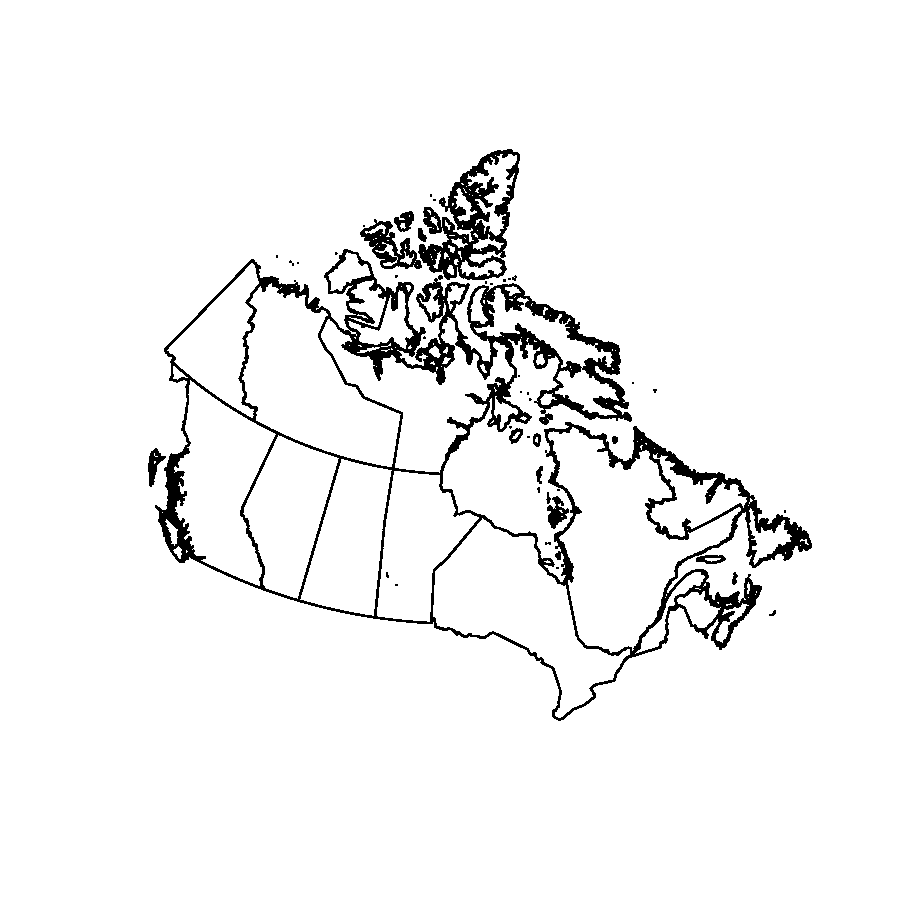
\includegraphics{hw03_bartschi-001}
{~\\\scriptsize It would appear that the graph is as it should be plotted, and there are 13 regions to be plotted.}

\item (4 Points)
Do some thinning and removal of very tiny islands (if necessary). The values
used in the China example may not be applicable for your country as they
depend on a given spatial coordinate system. You may have to considerably increase or
decrease the order of magnitude of these arguments.
Plot the final version of your thinned shapefile.

\begin{Schunk}
\begin{Sinput}
> CanadaShapefileThin <- thinnedSpatialPoly(CanadaShapefile, 
+                                          tolerance = 3000,
+                                          minarea =
+                                            10000000000,
+                                          topologyPreserve =
+                                            TRUE, 
+                                          avoidGEOS = TRUE)
> CanadaShapefileThin <- gBuffer(CanadaShapefileThin, 
+                                width = 0, 
+                                byid = TRUE)
> gIsValid(CanadaShapefileThin, byid = TRUE, reason = TRUE)
\end{Sinput}
\begin{Soutput}
               0                1                2                3 
"Valid Geometry" "Valid Geometry" "Valid Geometry" "Valid Geometry" 
               4                5                6                7 
"Valid Geometry" "Valid Geometry" "Valid Geometry" "Valid Geometry" 
               8                9               10               11 
"Valid Geometry" "Valid Geometry" "Valid Geometry" "Valid Geometry" 
              12 
"Valid Geometry" 
\end{Soutput}
\begin{Sinput}
> plot(CanadaShapefileThin)
\end{Sinput}
\end{Schunk}
\includegraphics{hw03_bartschi-002}

\item (4 Points)
Identify which variable contains the names or other identifiers for the spatial regions.
Find any online data for these regions. This could be population data, health data,
educational data, or whatever else you can find. Using {\it Wikipedia} is OK here.
Apply web scraping or manually enter the region names and values for these regions.
Show the head of the data frame of the data you selected.

\begin{Schunk}
\begin{Sinput}
> #Through a bit of trail and error, we discover
> CanadaShapefileThin$NAME_1 #contains the province names
\end{Sinput}
\begin{Soutput}
 [1] Alberta                   British Columbia         
 [3] Manitoba                  New Brunswick            
 [5] Newfoundland and Labrador Northwest Territories    
 [7] Nova Scotia               Nunavut                  
 [9] Ontario                   Prince Edward Island     
[11] Québec                   Saskatchewan             
[13] Yukon                    
13 Levels: Alberta British Columbia Manitoba ... Yukon
\end{Soutput}
\begin{Sinput}
> #to address an error with the names, we rename Quebec:
> levels(CanadaShapefileThin$NAME_1)[11] <- "Quebec"
> library(httr)
> library(XML)
> #Recived Data from Wikipedia page on Canada
> #Here we consider the population data from the 2015 census
> #Used URL Shortener to print full link on page:
> page <- GET("http://bit.ly/Canada_Population")
> # extract the nodes related to the tables
> pagehtml <- htmlParse(page)
> nodes <- getNodeSet(pagehtml, "//table")
> # extract the population table from the page
> etable <- readHTMLTable(nodes[[1]])
> colnames(etable) <- gsub(" |\n|[-]|[.]", "", 
+                          colnames(etable))
> Canada.pop <- data.frame(
+   province = etable$V2[3:15],
+   pop = as.integer(gsub(",", "", etable$V3[3:15]))
+ )
> head(Canada.pop)
\end{Sinput}
\begin{Soutput}
          province      pop
1          Ontario 13448494
2           Quebec  8164361
3 British Columbia  4648055
4          Alberta  4067175
5         Manitoba  1278365
6     Saskatchewan  1098352
\end{Soutput}
\end{Schunk}


\item (8 Points)
Create the map table and a basic linked micromap plot for your country,
based on code similar to the five to eight line--basic examples we 
used in class.
Just show a dotplot of the data in a single statistical panel.
Include a figure of your basic linked micromap plot, ideally written to
an external file and then incorporated back into R.

\begin{Schunk}
\begin{Sinput}
> CanadaPolys <- create_map_table(CanadaShapefileThin,
+                                 "NAME_1")
> CanadaPlot <- mmplot(stat.data = Canada.pop,
+                     map.data = CanadaPolys,
+                     panel.types = c("labels", 
+                                     "dot", "map"),
+                     panel.data = list("province", 
+                                       "pop", NA),
+                     ord.by = "pop",
+                     grouping = 3,
+                     median.row = TRUE, 
+                     map.link = c("province", "ID"))
\end{Sinput}
\end{Schunk}
\includegraphics{hw03_bartschi-004}


\item (5 Points)
Optimize your basic linked micromap plot and make it ready for publication.
Follow improvements from class, such as changing colors, adjusting axis labels,
adding reference lines (for national means or medians), etc.
Make sure to adjust the grouping to one of the recommendations from
Table~1.2 in {\it Symanzik\_Carr\_Handbook\_Proofs\_version3.pdf}
and include a median row if recommended in this table.
If you want, show more than a single statistical panel and select
a plot type other than a dotplot --- or just stay with a single statistical panel with a
dotplot. That's up to you (and the data you selected).
Include a figure of your final linked micromap plot, ideally written to
an external file and then incorporated back into R.

\begin{Schunk}
\begin{Sinput}
> library(RColorBrewer)
> CanadaPlot <- mmplot(stat.data = Canada.pop,
+                     map.data = CanadaPolys,
+                     panel.types = c("map", "dot_legend",
+                                     "labels", "dot"),
+                     panel.data = list(NA, NA, 
+                                       "province", "pop"),
+                     ord.by = "pop",
+                     grouping = c(4,5,4),
+                     rev.ord = TRUE,
+                     color = rev(brewer.pal(5, "GnBu")),
+                     two.ended.maps = TRUE,
+                     map.all = TRUE,
+                     map.color2 = "lightgray",
+                     map.link = c("province", "ID"),
+                     
+                     plot.header = 
+                       "Population of Canada by Region",
+       #For some reason, it doesn't include the title
+                     plot.header.size = 2,
+                     plot.header.color = "black",
+                     
+                     plot.panel.spacing = 0,
+                     panel.att = list(
+                       list(1, header = 
+                              "Two-ended\nCumulative Maps",
+                            inactive.border.color = 
+                              gray(.7), 
+                            inactive.border.size = 1,
+                            panel.width = 1.2),
+                       list(2, point.type = 20,
+                            point.size = 1.4),
+                       list(3, header = "Provinces", 
+                            panel.width = .9,
+                            align = "left", 
+                            text.size = .8),
+                       list(4, header = "Population",
+                            graph.bgcolor = "lightgray", 
+                            point.size = 1,
+                            xaxis.ticks = 
+                              seq(0, 14000000, 
+                                  by = 2000000), 
+                            xaxis.labels = 
+                              seq(0, 14, by = 2),
+                            xaxis.title = 
+                              "Number (Millions)"
+                       )
+                     )
+ )
\end{Sinput}
\end{Schunk}
\includegraphics{hw03_bartschi-005}

\end{enumerate}


\newpage


\item {\bf Overlay of Alabama Election Results from HW~2 on Street Map or Terrain Map}
(25 Points): \\
Create an overlay of your previously created map for the Alabama Election Results
on a street map or terrain map. Choose any R package that works for you.
If you work with {\it ggmap}, it may be easiest to ignore most of your 
work from HW~2 and reconsider how to use {\it ggplot} aesthetics (hint: the
winning intervals) for a far more elegant solution. The trick will be
to include a factor level for the unused interval for Jones.
If you work with {\it RgoogleMaps}, you should be able to reuse
most of your R code from HW~2. The Illinois example from the
{\it Choropleth Maps Overlays} section of our lecture notes may be helpful
for this question.

Do not forget to include a meaningful legend for all 10 intervals,
although only 9 are used in this map. If you wonder why this is
important, think of small multiples where you use the same colors
for several other states as well. While the Democratic candidate
did not win a single county with a percentage of 40\% to 50\% 
of the votes in Alabama, this may be the case in some counties
in other states. Thus, we should not omit this interval/color
from the Alabama legend.

Figure~\ref{AlabamaMap} shows an overlay on a Google map
from Spring 2018 when the Google map server could still be
freely accessed without a Google API key. Thus, your final
figure should be similar, but you won't be able to produce
exactly the same figure (unless you obtain a Google API key).

\begin{Schunk}
\begin{Sinput}
> ###Code from HW 2
> library(httr)
> library(XML)
> #Get the data, and transform it so that it is useful
> #Used URL shortener here as well, using original link:
> page <- GET("http://bit.ly/TimesALelection")
> pagehtml <- htmlParse(page)
> nodes <- getNodeSet(pagehtml, "//table")
> class(nodes)
\end{Sinput}
\begin{Soutput}
[1] "XMLNodeSet"
\end{Soutput}
\begin{Sinput}
> etable <- readHTMLTable(nodes[[2]])
> colnames(etable) <- gsub(" |\n|[-]|[.]", "", 
+                          colnames(etable))
> etable$JonesNum <- as.integer(gsub(",", "", etable$Jones))
> etable$MooreNum <- as.integer(gsub(",", "", etable$Moore))
> etable$WriteInsNum <- as.integer(gsub(",", "",
+                                       etable$WriteIns))
> etable$total.votes <- etable$JonesNum + 
+   etable$MooreNum + 
+   etable$WriteInsNum
> etable$Jones.Pct <- etable$JonesNum / etable$total.votes
> etable$Moore.Pct <- etable$MooreNum / etable$total.votes
> for(i in 1:length(etable$County)){
+   if(etable$Jones.Pct[i] > etable$Moore.Pct[i]){
+     etable$Moore.Pct[i] <- NA
+   } else {
+     etable$Jones.Pct[i] <- NA
+   }
+ }
> library(maps)
> winning.Pct <- vector(mode="numeric", 
+                       length=length(etable$County))
> etable.sorted <- etable[order(etable$County),]
> counties <- gsub("alabama,", "", 
+                  map("county","Alabama", plot = F)$names)
> alabama.breaks <- c(-.9,-.8,-.7,-.6,-.5, 0, 
+                     .5, .6, .7, .8, .9)
> for (i in 1:length(etable$County)){
+   if(is.na(etable.sorted$Jones.Pct[i])){
+     winning.Pct[i] <- -(etable.sorted$Moore.Pct[i])
+   } else{
+     winning.Pct[i] <- etable.sorted$Jones.Pct[i]
+   }
+ }
> m.winning <- cut(winning.Pct, alabama.breaks)
> par(mar=c(5.1, 4.1, 4.1, 8.1), xpd=TRUE)
> map.m.col <- brewer.pal(10, "RdBu")[m.winning]
> ###End of HW two code
> 
> library(RgoogleMaps)
> library(PBSmapping)
> library(maptools)
> library(maps)
> apiKey <- scan("C:/Users/Shaun/Desktop/BingMapKey.txt", 
+                what = "")
> al <- map("county", "Alabama", fill = TRUE,
+     col = map.m.col, border = "White", plot = FALSE)
> IDs <- sub("^alabama,", "", al$names)
> al_sp <- map2SpatialPolygons(al, IDs, 
+                               CRS("+proj=longlat"))
> bb <- qbbox(lon = coordinates(al_sp)[, 1], 
+             lat = coordinates(al_sp)[, 2])
> MyILMap <- GetBingMap(mapArea = c(bb$latR[1], 
+                                   bb$lonR[1], 
+                                   bb$latR[2], 
+                                   bb$lonR[2]), 
+                       maptype = "Road",
+                       apiKey = apiKey, 
+                       destfile = "IL.jpg", 
+                       verbose = 1)
\end{Sinput}
\begin{Soutput}
[1] "http://dev.virtualearth.net/REST/v1/Imagery/Map/Road?mapArea=30.7174855002758,-88.2748640793059,34.9249161908533,-85.1787782329056&mapSize=640,640&format=png&key=AoGO1DAMPe94nSbXD_nRVG3yup7ShQmhPByO1LjtZOGSNYXsQsNpF2AiAjRGyX2e"
\end{Soutput}
\begin{Sinput}
> #help with transparency from dataanalytics.org.uk
> #website: http://bit.ly/2J9H3cA
> rgb.map.col <- col2rgb(map.m.col)
> PlotPolysOnStaticMap(MyILMap, al_sp, lwd = 0.5, 
+                      col = rgb(rgb.map.col[1,], 
+                                rgb.map.col[2,], 
+                                rgb.map.col[3,],
+                                max = 255,
+                                alpha = (50*255/100)),
+                      add = FALSE, border = "White")
> title(main = "Alabama 2017 Special Election Results")
> legend("left", legend =
+          c("Rep 80-90%","Rep 70-80%","Rep 60-70%",
+            "Rep 50-60%","Rep <50%",
+            "Dem <50%","Dem 50-60%","Dem 60-70%",
+            "Dem 70-80%","Dem 80-90%"),
+        fill = brewer.pal(10, "RdBu"), 
+        title = "Winning Vote Share")
\end{Sinput}
\end{Schunk}
\includegraphics{hw03_bartschi-006}

\newpage


\begin{figure}[h]
\begin{center}
\includegraphics[width=0.95\textwidth]{hw03_alabama_google_historical.pdf}
\end{center}
\caption{\label{AlabamaMap}
County--by--county Outcome of the 2017 Alabama Special Election in the 
Doug Jones (Dem) vs.\ Roy Moore (Rep) Senate Race. The map shows the
winning percentage (in \%) in each of the 67 Alabama counties.}
\end{figure}


\newpage


\item {\bf Shiny App for Bad Color Graphic from HW~2} (25 Points): \\
Build a shiny app that allows a user to toggle between
the original graphic with the bad colors and a graphic with improved colors.
These should be your graphics / improvements from HW~2.

Moreover, add a 2nd selection mechanism that let's a user check for various
colorblind appearances of these graphics, i.e., the original and the improved one.
This should be based on the {\it dichromat} R package and the three
color--blindness types deutan, protan, and tritan.
Overall, your app should be able to show six differently colored graphics:
two sets of color (original and improved) $\times$ three types of color--blindness.
Include screenshots that show your shiny app and the resulting graphics
for all of these six settings.

Adding a toggle button that allows you to add/choose different symbols
or sizes (or what else you may have done in HW~2 to further improve
your original graph) is optional.

When you develop such an app, follow the principle from class:
Start with the most basic app that just shows your original bad graph
(the default). Then add one control option after the other.

Include only the final version of your R code. Make sure
that you change to \verb|eval=FALSE| for this question
when you compile your Rnw document.


\newpage


\item {\bf Using the Grand Tour for an Interactive Clustering} (25 Points): \\
Load the file {\it hw03\_mystery.csv} into {\it GGobi}, the {\it rggobi} R package, or any other
standalone software or R package that allows you to apply a {\bf brush--tour} strategy
as introduced in the {\it Grand Tour} section of our lecture notes.

{\bf I have asked our computer support people
to install {\it GGobi}/{\it rggobi} on one or two publicly accessible computers in
our department. If you are interested in working on this question,
but do not have access to {\it GGobi}/{\it rggobi} on your own computer,
you will hopefully be able to use one of the computers here in
the department within the next few days. I will post an announcement in Canvas
when {\it GGobi}/{\it rggobi} have been installed on a 
departmental computer.}

My instructions below are written under the assumption that you are using {\it GGobi}.

For this question, you do not have to include any R code.


\begin{enumerate}

\item (5 Points)
Start the grand tour and select the six variables called {\it V1, $\ldots$, V6}.
Do {\bf not} select the variable {\it Row}. In the grand tour window,
select {\it Options $\rightarrow$ Show Axes} to show the projection of the
variable axes. Adjust the speed of the tour as desired. 

First look for obvious outliers
in the grand tour. These are single points that behave rather differently from all
other points in the tour. Once you have spotted an outlier, stop the tour
and brush this point with a big red $X$. Continue and find the next outlier, etc.
There are $\geq 1$ and $\leq 5$ outliers. How many outliers did you find?

Continue the tour and find a projection where
all of your outliers are visible and well separated from the
other data points at the same time. Such a projection exists.
Do some fine adjustment of this projection with the mouse. Which 
variables contribute most to this projection? Also include a screenshot
(or photo taken with your phone) of this projection
as part of your answer. Make sure that the variable axes are visible. 


\item (4 Points)
Now focus on clusters via the grand tour. There are $\geq 2$ and $\leq 5$
clusters in this data set. Whenever you think you identified a cluster,
i.e., a group of points that moves in a different direction, persistently
brush it with a new color and symbol. 

If you paused the tour a fraction of a second too late, do some adjustment
of the projection with the mouse to get back to a more interesting projection.
Do not brush your previously detected
outliers again! 

After each new cluster you detected, take a screenshot (or photo)
and include it as part of your answer. As before, make sure that the 
variable axes are visible. How many main clusters did you detect? 


\item (4 Points)
Find a projection in the grand tour that separates your clusters and
the outliers reasonably well. There may not be a perfect projection
that separates all clusters and the outliers at the same time.

Also activate a parallel coordinate plot (PCP) and a scatterplot matrix of all
six variables and {\it Row}. Make sure that the variables
appear in the order {\it V1, $\ldots$, V6, Row}. If this is not the case
pull the axes in the PCP until they appear in the right place in {\it GGobi}.
For the scatterplot matrix, unselect variables and select them in the
proper order again in {\it GGobi}. Include a screenshot of the final projection
from the grand tour, the PCP, and the scatterplot matrix. 


\item (4 Points)
Revisit your outliers: What are the {\it Row} numbers for your outliers?
Note that {\it Identify} in {\it GGobi} provides you with the case number 
(or row label used by {\it GGobi}).
The {\it Row} number in our data set is the {\it GGobi} case number $+ 1$.
This becomes obvious in {\it Tools $\rightarrow$ Data Viewer}. 

Are you surprised how your outliers look in the PCP and the scatterplot matrix?
I would be $\ldots$ Is there a single axis in the PCP that would have
allowed you to detect a specific outlier (which outlier and which axis)? 
Is there any pairwise scatterplot in the scatterplot matrix that would have
allowed you to detect a specific outlier (which outlier and which pairwise scatterplot)? 
Using the variable axes information from the grand tour may help.

Verbally describe the characteristics of the outliers you detected. 


\item (4 Points)
Revisit your clusters: How many did you detect visually?
Are there any variables in the PCP that would have allowed you
to identify the same clusters? Which ones? Is this a clear separation?

Are there any pairwise scatterplots in the scatterplot matrix that would have
allowed you to detect the same clusters? Which ones? Is this a clear separation?
When you refer to your clusters, identify them by the colors and glyphs
you used, e.g., the cluster made up by the ``yellow o'' and the cluster 
made up by the ``purple $+$''. 


\item (4 Points)
Overall, did we benefit from the grand tour, or could we just have used
a PCP and/or a scatterplot matrix? Be specific and justify your answer.
Compare which variable axes had most impact in the screenshots (or photos) you created
from the grand tour with subsets of these variables in the PCP and in the
pairwise scatterplots. 


\end{enumerate}


\end{enumerate}


\newpage


\noindent{\Large \bf General Instructions}~\\


\begin{enumerate}
\item Create a single pdf document, using R Markdown, Sweave, or knitr.
When you take this course at the 6000--level, you have to use \LaTeX\ in
combination with Sweave or knitr.
You only have to submit this one document.

\item Include a title page that contains your name, your A--number, the number of
the assignment, the submission date, and any other relevant information.

\item Start your answers to each main question on a new page (continuing with the next
part of a question on the same page is fine). 
Clearly label each question and question part.

\item Show your R code for each question part!

\item Before you submit your homework, check that you
follow all recommendations from Google's R Style Guide
(see \url{https://google.github.io/styleguide/Rguide.xml}). 
Moreover, make sure that your R code is consistent, i.e., that you use the same
type of assignments and the same type of quotes throughout your entire homework.

\item Give credit to external sources, such as stackoverflow or help pages. Be specific
and include the full URL where you found the help (or from which help page you got 
the information). Consider R code from such sources as ``legacy code or third--party code'' 
that does not have to be adjusted to Google's R Style (even though it would be nice,
in particular if you only used a brief code segment).

\item {\bf Not following the general instructions outlined above will result in point deductions!}

\item For general questions related to this homework, please
use the corresponding discussion board in Canvas! I will try to
reply as quickly as possible. Moreover, if one of you knows
an answer, please post it. It is fine to refer to web pages
and R commands, but do not provide the exact R command with all required arguments
or which of the suggestions from a stackoverflow web page eventually worked for you! 
This will be the task for each individual student!

\item Submit your single pdf file via Canvas by the submission deadline.
Late submissions will result in point deductions as outlined on the syllabus.

\end{enumerate}


\end{document}

